\section{Bilateral Filter}


The depthmaps captured by a low cost RGB-D camera usually contains noise, this can be 
consecuence of materials reflectance, device imperfections, object fast movement, distance to the 
sensor, etc. 

In order to reduce the effect of noise is natural to use some kind of filter, as usual in computer 
vision, a typical filter will take information of a pixel and its neighboorhod to generate a result. 
If the image is smooth, without abrupt changes in intensity, a simple average could be enough. However, this 
is not the case in the presence of edges or corners, areas where the intensity changes charply. 
The bilateral filter afronts this problem, giving to each neighboor a weight based on its cercany  
to the center pixel. In a grayscale image it takes into account 
the neighboor intensity distance and location distance (in image plane) to calculate the weight.  A depthmap is very similar to a grayscale 
image, the only difference is that the depth map represents geometrical information and usually contains holes 
(areas where the sensor failed to capture distance). 

A bileateral filter was applied to the depth maps, using the euclidean distance and z axis distance to calculate 
the weight of each pixel neighboor in the depth map.

In a filter window centered at pixel location $(x,y)$, the ponderated average was calculated using the following weight for each neighboor:

$$ kernel(v,\sigma) = \frac{e^{-v^2}}{2*\sigma^2} $$

$$ weight = kernel(d,\sigma_d)*kernel(z,\sigma_z) $$

Where 

$$ d = ||p - q|| $$
$$ z = |p_z - q_z| $$
$$ p = 3Dproj(x,y) = (p_x,p_y,p_z) $$ 
$$ q = 3Dproj(x_q,y_q) = (q_x,q_y,q_z) $$

The pixel p is the central pixel and the pixel q is one of its neighboors. Each pixel has a $weight$ that depends on its euclidean and z axis distance to the central pixel. The parameter $\sigma_d$ defines 
the neighborhood, all points of the depthmap that are at euclidean distance $2*\sigma_d$ or less from the central pixel are considered.

The final value of the center pixel is then

$$z = \frac{1}{totalWeight}\sum\limits_{k=1}^N{weight_k*z_k}$$
$$totalWeight = \sum\limits_{k=1}^N {weight_k}$$

Where N is the size of the pixel neighborhood (amount of points at an euclidean distance less than $2*\sigma_d$)  plus 1.

After applying this filter we obtain an smoothed version of the depth map, without loosing edges and important geometrical information.
A detailed explanation of the bilateral filter can be found in \cite{TomasiBilateral}.

\begin{figure}[h!]
\begin{center}
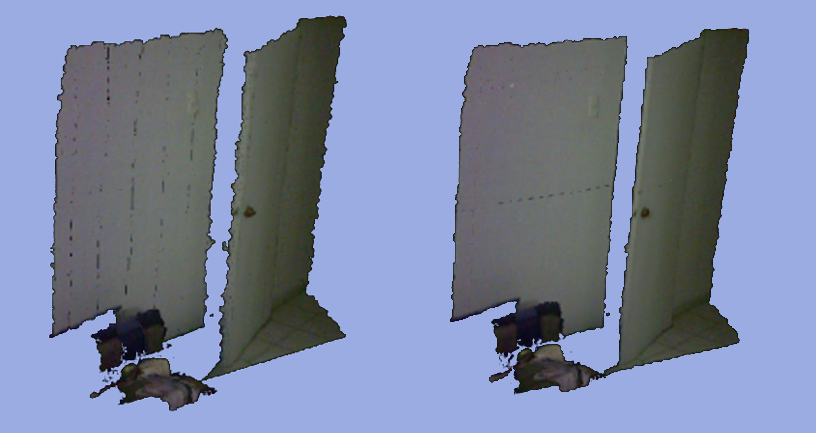
\includegraphics[scale=0.35]{images/bilateral}
\end{center}
\caption{Left: Point cloud without filtering Right: Point cloud with bilateral filtering. Noticeable effects at first sight next to the borders of objects}
\end{figure}

